\documentclass[letterpaper]{article}
\title{Lab1 Report }
\date{Due: Mar 13th 3017}
\usepackage[margin=1in]{geometry}
\usepackage{amsmath}
\usepackage{amssymb}
\usepackage{url}
\usepackage{graphicx}
\usepackage{color}
\usepackage{algorithmic}
\usepackage{caption}
\usepackage{subcaption}

\author{Shiyu Feng, Ep Pravitra, and Marcus Pereira}

\begin{document}

\maketitle

\section{Gradient Descent on Squared Loss}

\subsection{Algorithm}
We define the loss function to be
\begin{align}
l_i (t) &= ||W_t f_i - y_i||^2
\end{align}
where $f_i \in  \mathbb{R}^{10}$ is a feature vector given by the problem.  $W \in  \mathbb{R}^{5x10}$ is the weight matrix that we seek to learn. $y_i \in  \mathbb{R}^5$ is an indicator vector corresponds to each label. We remap the labels to be.
\begin{itemize}
\item Veg : $y = [ \ 1 \ 0 \ 0 \ 0 \ 0 \ ]^T$
\item Wire :$y = [ \ 0 \ 1 \ 0 \ 0 \ 0 \ ]^T$
\item Pole : $y = [ \ 0 \ 0 \ 1 \ 0 \ 0 \ ]^T$
\item Ground : $y = [ \ 0 \ 0 \ 0 \ 1 \ 0 \ ]^T$
\item Facade : $y = [ \ 0 \ 0 \ 0 \ 0 \ 1 \ ]^T$
\end{itemize}
We use the update law.
\begin{align}
W_{t+1} &= W_t - \alpha  \frac{d l}{d W}
\end{align}
where 
\begin{align}
 \frac{d l}{d W} &= 2(W_t f_i - y_i) f_i
\end{align}
We choose the learning rate $\alpha = \frac{1}{\sqrt{T}}$. Our algorithm reshuffles the given data and pass them through the learning algorithm several times.  

\subsection{Results}
We implement the result using C++ and Qt framework. We use OpenGL for visualization. The result of classification after learning both datasets are shown in Fig. \ref{fig:learned1} and Fig. \ref{fig:learned2}.
\begin{figure}
  \centering
  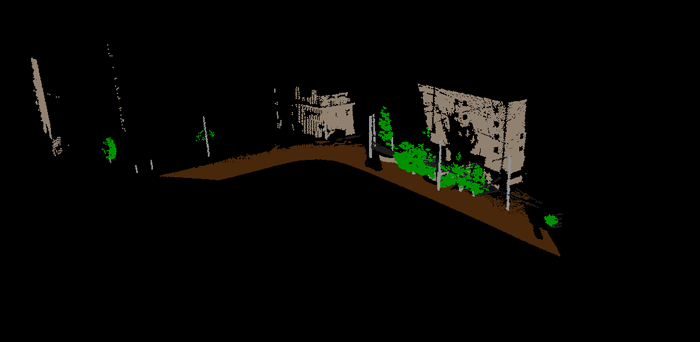
\includegraphics[scale = 0.4]{raw1}
\caption{given Dataset 1}
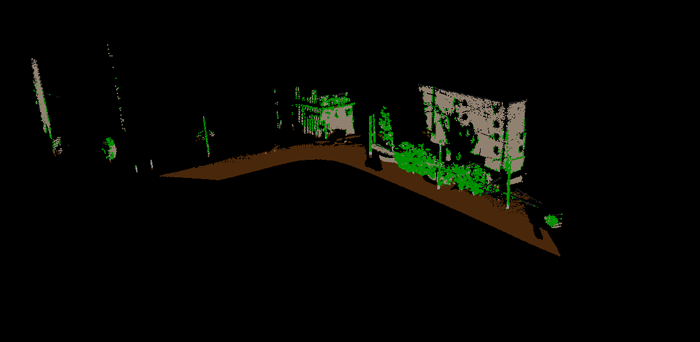
\includegraphics[scale = 0.4]{learned1}
\caption{classified Dataset 1}
\label{fig:learned1}
  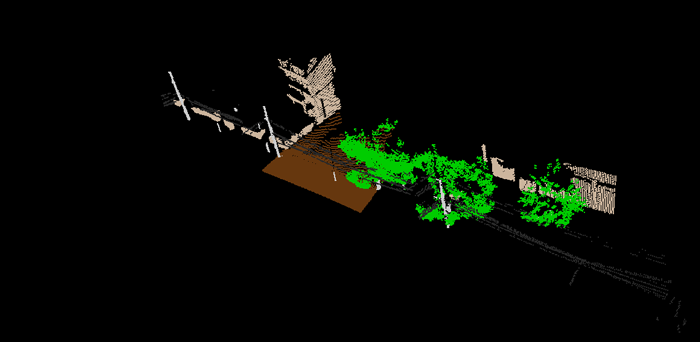
\includegraphics[scale = 0.4]{raw2}
\caption{given Dataset 2}
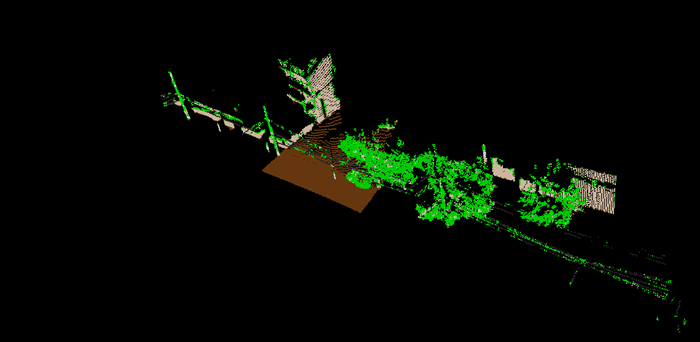
\includegraphics[scale = 0.4]{learned2}
\caption{classified Dataset 2}
\label{fig:learned2}
\end{figure}
 Here we show classification after 10 passes of both datasets. However, we discovered that passing datasets twice is already sufficient to obtain a consistent W. There is very little difference in outcome between 2 and 10 passes. 

\pagebreak

Fig. \ref{fig:learned1_apply2} shows another test case. In this case, we learn with Dataset 1 and use W to classify Dataset 2.\\

Wires and poles do not get classified very well for many potential reasons. One reason is they are consideraly "thinner features". Poles and wires have very little feature content in transverse direction. Other features are easier to classify because they tend to be clumped together. Size, density, and color information of clumped features are easier to extract.  We also note that we have much less samples of poles and wires in the  training set. This is especially true in our second test case where we learn using Dataset 1 (which do not have many wires) and attempt classify Dataset 2. Fig. \ref{fig:learned1_apply2} shows that wires are classified very poorly. \\

As often the case, choice of implemention is a direct tradeoff between implementation difficulty and CPU time. Our choice of C++ makes the learning and classification very fast. However, some implementation such as matrix multiplication is not trivial. Overall the algorithm is not difficult to implement.

\begin{figure}[h]
  \centering
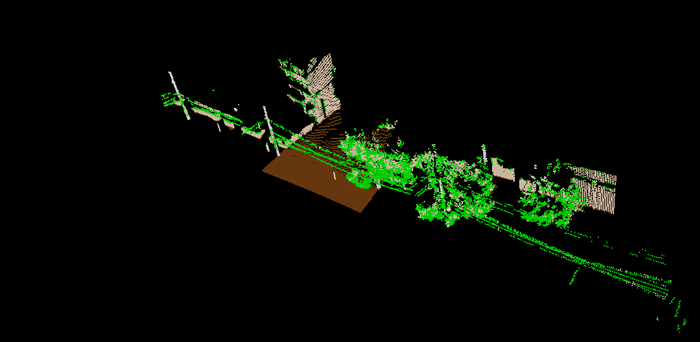
\includegraphics[scale = 0.4]{learned1_apply2}
\caption{classification of Dataset 2 by learning Dataset 1}
\label{fig:learned1_apply2}
\end{figure}

To evaluate robustness of the learned data, we apply $1 \sigma$ noise into Dataset 2. The classification result is shown in Fig \ref{fig:addnoiseto2}. Despite many misclassifications, facade and ground are still mostly correctly classified .

\begin{figure}[h]
  \centering
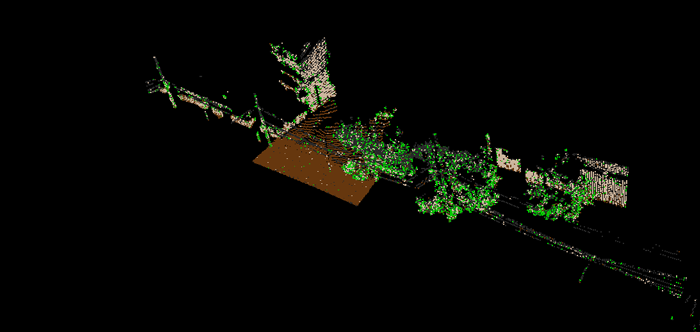
\includegraphics[scale = 0.4]{addnoiseto2}
\caption{classification results after noisy Dataset 2}
\label{fig:addnoiseto2}
\end{figure}
\end{document}
